\documentclass[tikz,border=0pt]{standalone}
\usepackage[T1]{fontenc}
\usepackage{newtxtext,newtxmath}
\usepackage{xcolor}
\definecolor{hbm}{HTML}{326C9B}
\definecolor{cpu}{HTML}{6D9FAD}
\definecolor{ink}{HTML}{203244}
\definecolor{rule}{HTML}{DFE6EC}
\begin{document}
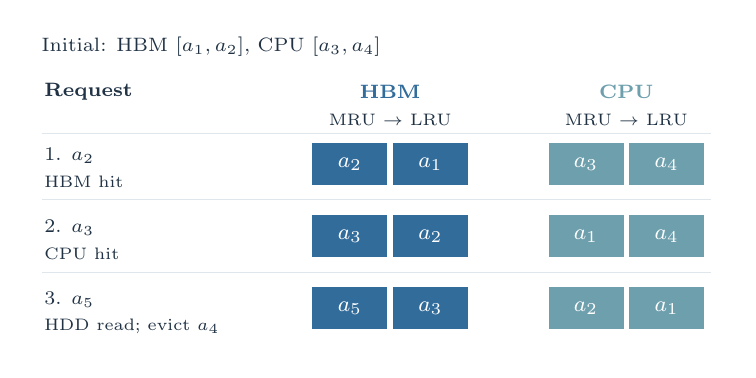
\begin{tikzpicture}[x=1bp,y=-1bp,every node/.style={inner sep=0pt,outer sep=0pt,text=ink,font=\fontsize{7.2}{8.4}\selectfont}]
\path[use as bounding box] (0,0) rectangle (252,115.92);
\node[anchor=west,font=\fontsize{7.5}{9}\selectfont] at (5,7)
  {Initial: HBM $[a_1,a_2]$, CPU $[a_3,a_4]$};
\node[anchor=west,font=\fontsize{7.5}{9}\selectfont\bfseries] at (6,23) {Request};
\node[text=hbm,font=\fontsize{7.5}{9}\selectfont\bfseries] at (130.5,23) {HBM};
\node[text=cpu,font=\fontsize{7.5}{9}\selectfont\bfseries] at (215.5,23) {CPU};
\node[font=\fontsize{6.5}{7.5}\selectfont] at (130.5,33) {MRU $\rightarrow$ LRU};
\node[font=\fontsize{6.5}{7.5}\selectfont] at (215.5,33) {MRU $\rightarrow$ LRU};
\draw[rule,line width=.35bp] (5,38) -- (246,38);
\draw[rule,line width=.3bp] (5,62) -- (246,62);
\draw[rule,line width=.3bp] (5,88) -- (246,88);
\node[anchor=west] at (6,46) {1. $a_2$};
\node[anchor=west,font=\fontsize{6.5}{7.5}\selectfont] at (6,55.5) {HBM hit};
\fill[hbm] (102.5,41.5) rectangle (129.5,56.5);
\node[text=white,font=\fontsize{8}{8}\selectfont] at (116,49) {$a_2$};
\fill[hbm] (131.5,41.5) rectangle (158.5,56.5);
\node[text=white,font=\fontsize{8}{8}\selectfont] at (145,49) {$a_1$};
\fill[cpu] (187.5,41.5) rectangle (214.5,56.5);
\node[text=white,font=\fontsize{8}{8}\selectfont] at (201,49) {$a_3$};
\fill[cpu] (216.5,41.5) rectangle (243.5,56.5);
\node[text=white,font=\fontsize{8}{8}\selectfont] at (230,49) {$a_4$};
\node[anchor=west] at (6,72) {2. $a_3$};
\node[anchor=west,font=\fontsize{6.5}{7.5}\selectfont] at (6,81.5) {CPU hit};
\fill[hbm] (102.5,67.5) rectangle (129.5,82.5);
\node[text=white,font=\fontsize{8}{8}\selectfont] at (116,75) {$a_3$};
\fill[hbm] (131.5,67.5) rectangle (158.5,82.5);
\node[text=white,font=\fontsize{8}{8}\selectfont] at (145,75) {$a_2$};
\fill[cpu] (187.5,67.5) rectangle (214.5,82.5);
\node[text=white,font=\fontsize{8}{8}\selectfont] at (201,75) {$a_1$};
\fill[cpu] (216.5,67.5) rectangle (243.5,82.5);
\node[text=white,font=\fontsize{8}{8}\selectfont] at (230,75) {$a_4$};
\node[anchor=west] at (6,98) {3. $a_5$};
\node[anchor=west,font=\fontsize{6.5}{7.5}\selectfont] at (6,107.5) {HDD read; evict $a_4$};
\fill[hbm] (102.5,93.5) rectangle (129.5,108.5);
\node[text=white,font=\fontsize{8}{8}\selectfont] at (116,101) {$a_5$};
\fill[hbm] (131.5,93.5) rectangle (158.5,108.5);
\node[text=white,font=\fontsize{8}{8}\selectfont] at (145,101) {$a_3$};
\fill[cpu] (187.5,93.5) rectangle (214.5,108.5);
\node[text=white,font=\fontsize{8}{8}\selectfont] at (201,101) {$a_2$};
\fill[cpu] (216.5,93.5) rectangle (243.5,108.5);
\node[text=white,font=\fontsize{8}{8}\selectfont] at (230,101) {$a_1$};
\end{tikzpicture}
\end{document}
